\documentclass{standalone}
\usepackage{tikz}
\usepackage{pgfplots}
\pgfplotsset{compat=newest}
\usepackage{pgfmath}
\usepackage{tikz-cd}
\usepackage{pgffor}
\usepackage{tkz-euclide}
\usetkzobj{all}
\usepgfplotslibrary{fillbetween}
\usetikzlibrary{
	calc,
	angles,
	quotes,
	arrows.meta,
	decorations.markings,
	math,
	backgrounds,
	pgfplots.statistics,
	matrix,
	patterns,
	shapes.geometric,
	spy,
	intersections,
}
\begin{document}
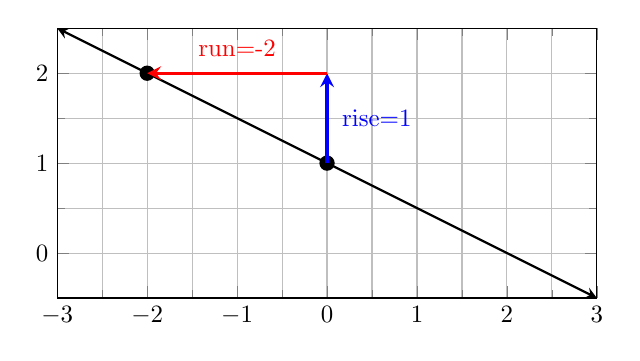
\begin{tikzpicture}[scale=1, every node/.style={scale=0.9}]
\begin{axis}[
    grid=both,
    unit vector ratio=1 1 1,
    ymin=-0.5,
    ymax=2.5,
    xmax=3,
    xmin=-3,
    xtick={-3,-2,...,3},
    ytick={-3,-2,...,4},
    minor tick num=1
]
\addplot[thick, samples=100,domain=-3:3, name path=A, stealth-stealth]   {-1/2*x+1};
\node[draw,shape=circle, minimum size=2mm,inner sep=0pt,outer sep=0pt, fill=black] at (0,1) {};
\node[draw,shape=circle, minimum size=2mm,inner sep=0pt,outer sep=0pt, fill=black] at (-2,2) {};
\addplot[blue, draw, -stealth, very thick] (0, 1)--(0,2) node[midway, xshift=2em] {rise=1};
\addplot[red, draw, -stealth, very thick] (0, 2)--(-2,2) node[midway, yshift=1em] {run=-2};
\end{axis}
\end{tikzpicture}
\end{document}